\RequirePackage{fix-cm}
%
\RequirePackage{amsmath}



%\documentclass{svjour3}                     % onecolumn (standard format)
%\documentclass[smallcondensed]{svjour3}     % onecolumn (ditto)
%\documentclass[smallextended]{svjour3}       % onecolumn (second format)
% \documentclass[twocolumn]{svjour3}          % twocolumn
%\documentclass[letterpaper, 12pt, twocolumn]{article}
\documentclass{article}
\usepackage[cm]{fullpage}
%\usepackage[margin=1in]{geometry}
\usepackage{amssymb}
\usepackage{graphicx}
\usepackage[utf8]{inputenc}
\usepackage{indentfirst}
%\usepackage{physics}
\newcommand{\me}{\mathrm{e}}
\usepackage{amsmath}

%\usepackage[monochrome]{color}

%\usepackage[round]{natbib}
%\usepackage{apacite}
\usepackage{url}


\PassOptionsToPackage{monochrome}{xcolor}

% For the flow charts
\usepackage{tikz}
\usetikzlibrary{
	external,
}
\tikzexternalize

\usetikzlibrary{shapes.geometric, arrows, calc, positioning}
\tikzstyle{startstop} = [rectangle, thick, rounded corners=2.5mm, minimum width=2cm, minimum height=5mm,text centered, draw=black]
\tikzstyle{io} = [trapezium, thick, trapezium left angle=70, trapezium right angle=110, text width=3.75cm, minimum height=0.5cm, text centered, draw=black]
\tikzstyle{process} = [rectangle, thick, minimum width=2.5cm, text width=4cm, minimum height=0.5cm, text centered, draw=black]
\tikzstyle{block} = [rectangle, thick, minimum width=0.5cm, minimum height=1cm, text centered, draw=black]
\tikzstyle{support} = [coordinate, join=by fuzzy]
\tikzstyle{decision} = [diamond, thick, minimum width=3cm, minimum height=1cm, text centered, draw=black]
\tikzstyle{dottedbox} = [rectangle, dotted, thick, minimum width=2.5cm, text width=2.8cm, minimum height=0.5cm, text centered, draw=black]
\tikzstyle{arrow} = [thick,->,>=stealth]
\tikzstyle{dottedarrow} = [thick, dotted,->,>=stealth]





\usepackage{pgfplots}
\usepgfplotslibrary{patchplots}
\pgfplotsset{compat=newest, samples=015} %Set this value to 65 for the final version
%\usepgfplotslibrary{dateplot} 


%\providecommand{\keywords}[1]{\textbf{\textit{Index terms---}} #1}

%\journalname{Journal of Science Education and Technology}

\begin{document}
	
	
	\title{Diagrams for the android app Control Toolbox (Continuous time)}

\begin{figure}
\centering
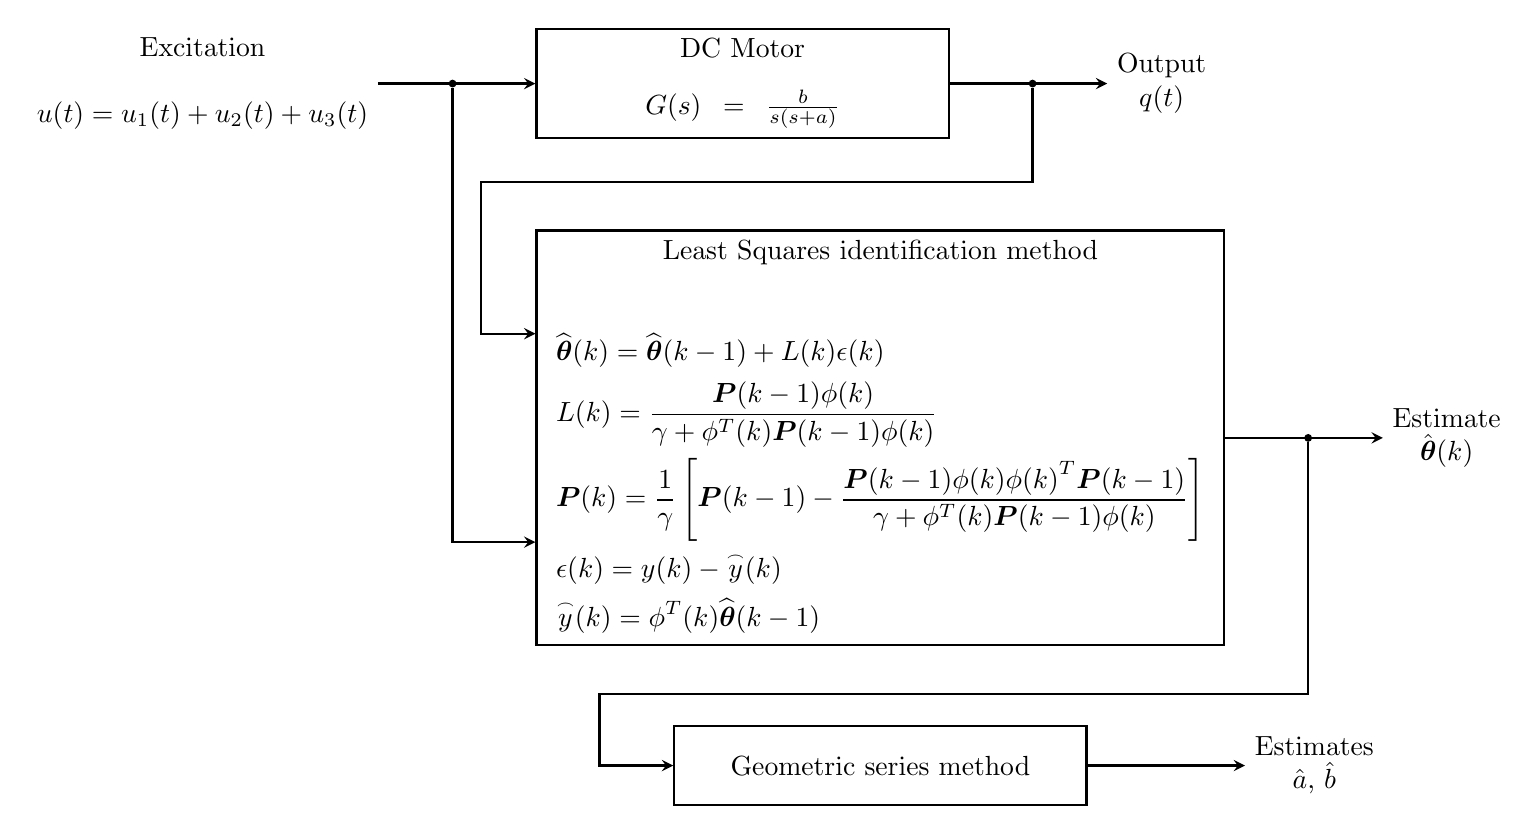
\begin{tikzpicture}[node distance = 10mm, auto]
	\node (Excitation) [align=center] {Excitation\\\\$u(t)=u_1(t)+u_2(t)+u_3(t)$};
	\node (Plant) [block, text width = 5cm, right = of Excitation, right = 2cm] {DC Motor \\[0.3cm] $G(s) = \frac{b}{s(s+a)}$};
	\node (PlantRight) [support, right = of Plant, right = 1cm, fill,circle,scale=0.3] {};
	\node (PlantLeft) [support, left = of Plant, left = 1cm, fill,circle,scale=0.3] {};
	\node (Identification) [block, text width = 8.5cm, below = 4.5 of Plant.west, anchor=west] {Least Squares identification method
		\\[0.1cm]
		\begin{align}
			& \widehat{\boldsymbol{\theta }}(k)=\widehat{\boldsymbol{\theta }}(k-1)+L(k)\epsilon (k) \nonumber\\
			& L(k)=\frac{\boldsymbol{P}(k-1)\phi (k)}{\gamma +{{\phi }^{T}}(k)\boldsymbol{P}(k-1)\phi (k)} \nonumber\\ 
			& \boldsymbol{P}(k)=\frac{1}{\gamma }\left[ \boldsymbol{P}(k-1)-\frac{\boldsymbol{P}(k-1)\phi (k)\phi {{(k)}^{T}}\boldsymbol{P}(k-1)}{\gamma +{{\phi }^{T}}(k)\boldsymbol{P}(k-1)\phi (k)} \right] \nonumber\\ 
			& \epsilon (k)=y(k)-\overset{\scriptscriptstyle\frown}{y}(k) \nonumber\\ 
			& \overset{\scriptscriptstyle\frown}{y}(k)={{\phi }^{T}}(k)\widehat{\boldsymbol{\theta }}(k-1)  \nonumber
		\end{align}
		
	};
	\node (IdentificationRight) [support, right = of Identification, right = 1cm, fill,circle,scale=0.3] {};
	\node (Geo) [block, text width = 5cm, below = 1 of Identification] {Geometric series method};
	\node (GeoOut) [right = of Geo, right = 2cm, align=center] {Estimates\\$\hat a$, $\hat b$};
	\node (Output) [right = of Plant, right = 2cm, align=center] {Output\\$q(t)$};
	\node (CapValues) [right = of Identification, right = 2cm, align=center] {Estimate\\$\hat{\boldsymbol{\theta}}(k)$};
	\path (Excitation.east) -- (Excitation.north east) coordinate[pos=0.5] (Reference1);
	\path (Identification.west) -- (Identification.north west) coordinate[pos=0.5] (Identification1);
	\path (Identification.west) -- (Identification.north west) coordinate[pos=-0.5] (Identification2);
	\path (Geo.west) -- (Geo.north west) coordinate[pos=0.0] (Geo1);
	\draw [arrow] (Excitation) -- (Plant);
	\draw [arrow] (Plant) -- (Output);
	\draw [arrow] (PlantRight) -- +(0, -1.25) -| +(-7,-1.25) |- (Identification1);
	\draw [arrow] (IdentificationRight) -- +(0, -3.25) -| +(-9,-3.25) |- (Geo1);
	\draw [arrow] (PlantLeft) |- (Identification2);
	\draw [arrow] (Identification) -- (CapValues);
	\draw [arrow] (Geo) -- (GeoOut);
	
\end{tikzpicture}
\caption{Identification of the DC motor parameters}
\end{figure}

\begin{figure}
\centering
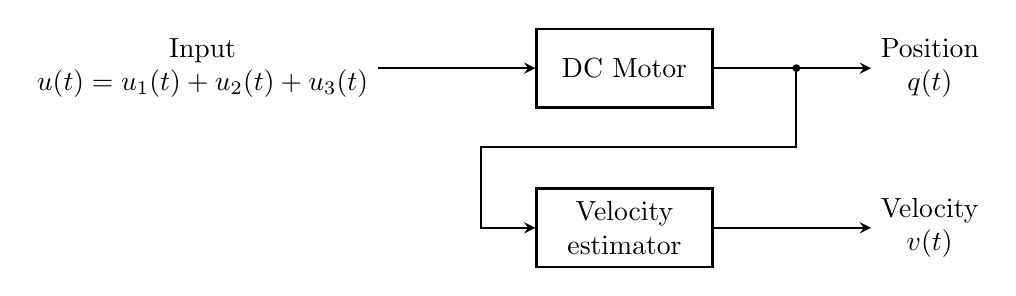
\begin{tikzpicture}[node distance = 10mm, auto]
	\node (Input) [align=center] {Input\\$u(t)=u_1(t)+u_2(t)+u_3(t)$};
	\node (Plant) [block, text width = 2cm, right = 2cm of Input] {DC Motor};
	\node (Output) [right = of Plant, right = 2cm, align=center] {Position\\$q(t)$};
	\node (VelEst) [block, text width = 2cm, below = 1 of Plant] {Velocity\\estimator};
	\node (VelOut) [right = of VelEst, right = 2cm, align=center] {Velocity\\$v(t)$};
	\node (PlantRight) [support, right = of Plant, right = 1cm, fill,circle,scale=0.3] {};
	\path (VelEst.west) -- (VelEst.north west) coordinate[pos=0.0] (VelEst1);
	\draw [arrow] (Input) -- (Plant);
	\draw [arrow] (Plant) -- (Output);
	\draw [arrow] (VelEst) -- (VelOut);
	\draw [arrow] (PlantRight) -- +(0, -1) -| +(-4,-1) |- (VelEst1);
\end{tikzpicture}
\caption{Open loop system}
\end{figure}






\begin{figure}
\centering
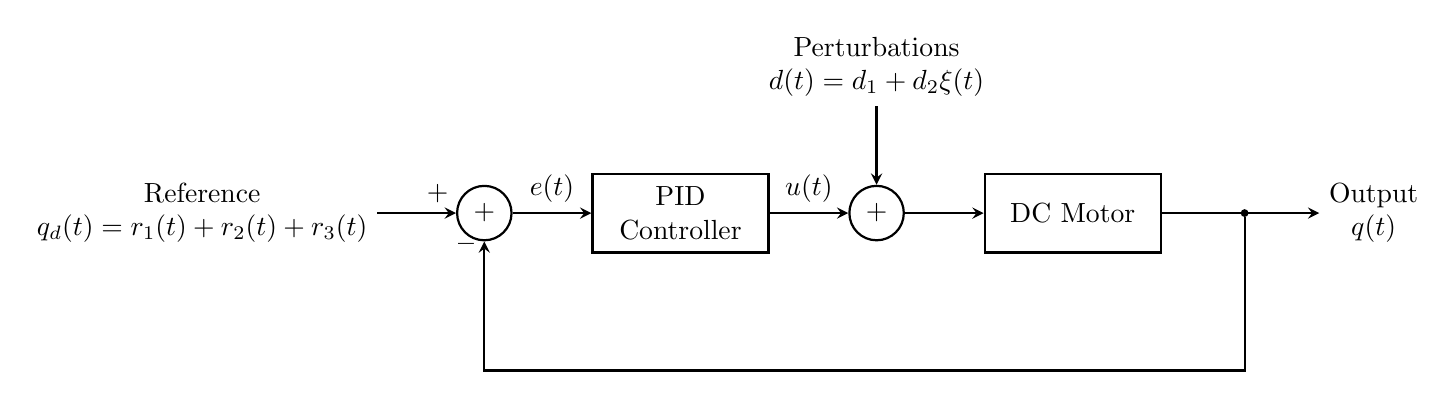
\begin{tikzpicture}[node distance = 10mm, auto]
	\node (Reference) [align=center] {Reference\\$q_d(t)=r_1(t)+r_2(t)+r_3(t)$};
	\node (SummingPoint) [draw,circle, thick, right = of Reference]  {+};
	\node (Control) [block, text width = 2cm, right = of SummingPoint] {PID Controller};
	\node (SummingPoint1) [draw,circle, thick, right = of Control]  {+};
	\node (Plant) [block, text width = 2cm, right = of SummingPoint1] {DC Motor};
	\node (PlantRight) [support, right = of Plant, right = 1cm, fill, circle,scale=0.3] {};
	\node (Output) [right = of Plant, right = 2cm, align=center] {Output\\$q(t)$};
	\node (Perturbations) [align=center, above = of SummingPoint1] {Perturbations\\$d(t)=d_1+d_2\xi(t)$};
	\draw [arrow] (Reference) -- node[anchor=south west]{+}(SummingPoint);
	\draw [arrow] (SummingPoint) -- node[anchor=south]{$e(t)$}(Control);
	\draw [arrow] (Control) -- node[anchor=south]{$u(t)$}(SummingPoint1);
	\draw [arrow] (SummingPoint1) -- (Plant);
	\draw [arrow] (Plant) -- (Output);
	\draw [arrow] (PlantRight) -- +(0, -2) -| (SummingPoint) node[below = 2mm, anchor=north east]{\bf\textendash};
	\draw [arrow] (Perturbations) -- (SummingPoint1);
\end{tikzpicture}
\caption{Closed loop system with a PID Controller}
\end{figure}


\begin{figure}
\centering
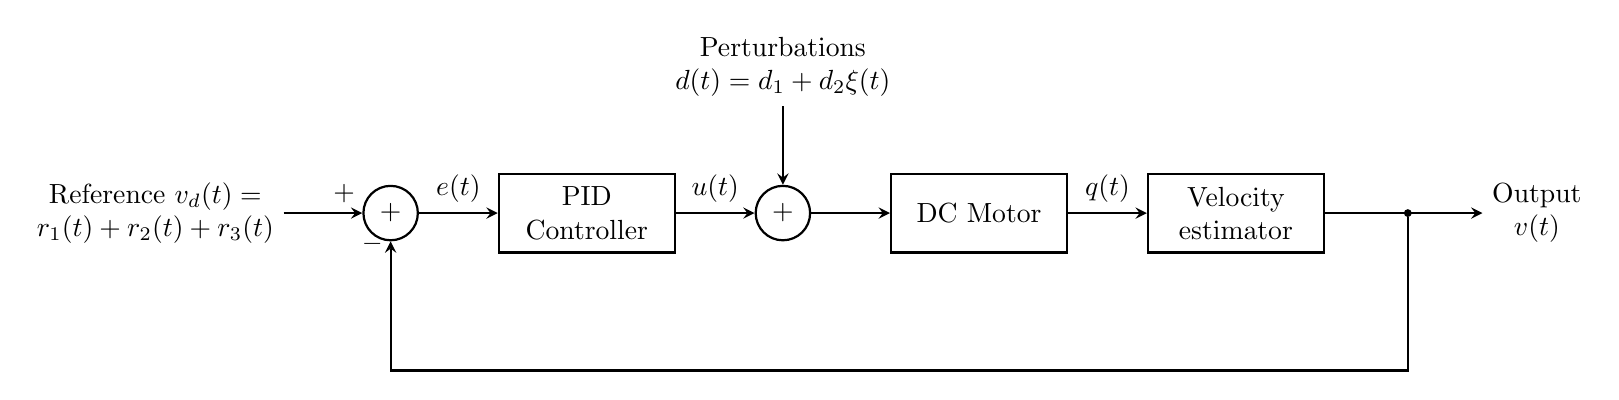
\begin{tikzpicture}[node distance = 10mm, auto]
	\node (Reference) [align=center] {Reference $v_d(t)=$\\$r_1(t)+r_2(t)+r_3(t)$};
	\node (SummingPoint) [draw,circle, thick, right = of Reference]  {+};
	\node (Control) [block, text width = 2cm, right = of SummingPoint] {PID Controller};
	\node (SummingPoint1) [draw,circle, thick, right = of Control]  {+};
	\node (Plant) [block, text width = 2cm, right = of SummingPoint1] {DC Motor};
	\node (VelEst) [block, text width = 2cm, right = of Plant] {Velocity\\estimator};
	\node (VelRight) [support, right = of VelEst, right = 1cm, fill, circle,scale=0.3] {};
	\node (Output) [right = of VelEst, right = 2cm, align=center] {Output\\$v(t)$};
	\node (Perturbations) [align=center, above = of SummingPoint1] {Perturbations\\$d(t)=d_1+d_2\xi(t)$};
	\draw [arrow] (Reference) -- node[anchor=south west]{+}(SummingPoint);
	\draw [arrow] (SummingPoint) -- node[anchor=south]{$e(t)$}(Control);
	\draw [arrow] (Control) -- node[anchor=south]{$u(t)$}(SummingPoint1);
	\draw [arrow] (SummingPoint1) -- (Plant);
	\draw [arrow] (Plant) -- node[anchor=south]{$q(t)$}(VelEst);
	\draw [arrow] (VelEst) -- (Output);
	\draw [arrow] (VelRight) -- +(0, -2) -| (SummingPoint) node[below = 2mm, anchor=north east]{\bf\textendash};
	\draw [arrow] (Perturbations) -- (SummingPoint1);
\end{tikzpicture}
\caption{Closed loop system with a PID Controller}
\end{figure}



\begin{figure}
\centering
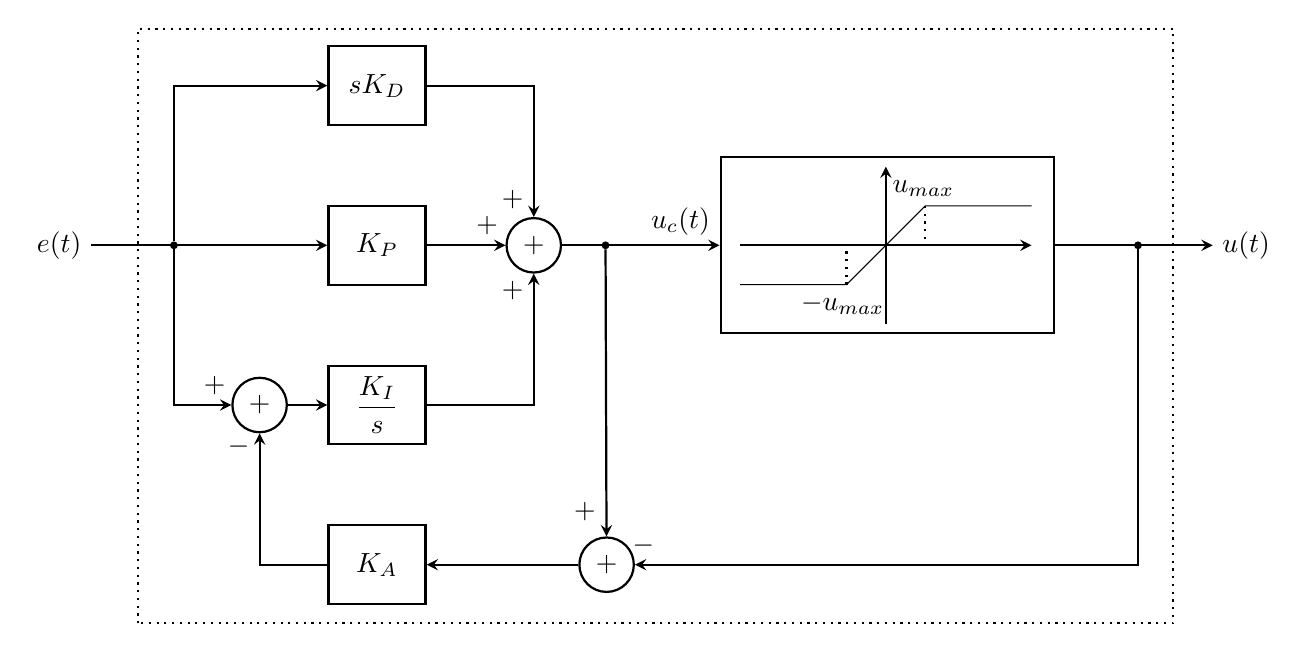
\begin{tikzpicture}[node distance = 10mm, auto]
	\node (Error) [align=center] {$e(t)$};
	\node (KP) [block, text width = 1cm, right = 3cm of Error] {$K_P$};
	\node (KD) [block, text width = 1cm, above = of KP] {$sK_D$};
	\node (KI) [block, text width = 1cm, below = of KP] {$\dfrac{K_I}{s}$};
	\node (KA) [block, text width = 1cm, below = of KI] {$K_A$};
	\node (SummingPoint0) [draw,circle, thick, right = of KP]  {+};
	\node (SummingPoint1) [draw,circle, thick, left = 0.5cm of KI]  {+};
	\node (SummingPoint2) [draw,circle, thick, right = 1.925cm of KA]  {+};
	\node (Sat) [block, text width = 4cm, text height = 2cm, right = 2cm of SummingPoint0] {};
	\node (Out) [align=center, right = 2cm of Sat] {$u(t)$};
	\node (ErrorRight) [support, right = of Error, right = 1cm, fill, circle,scale=0.3] {};
	\node (SummingPoint0Right) [support, right = of SummingPoint0, right = 0.5cm, fill, circle,scale=0.3] {};
	\node (SatRight) [support, right = of Sat, right = 1cm, fill, circle,scale=0.3] {};
	\draw [arrow] (Error) -- (KP);
	\draw [arrow] (ErrorRight) |- (KD);
	\draw [arrow] (ErrorRight) |- node[right = 0.25cm, anchor=south west]{$+$}(SummingPoint1);
	\draw [arrow] (SummingPoint1) -- (KI);
	\draw [arrow] (KA) -| node[above = 1.75cm, anchor=north east]{$-$}(SummingPoint1);
	\draw [arrow] (KP) -- node[anchor=south west]{$+$}(SummingPoint0);
	\draw [arrow] (KD) -| node[below=1.2cm, anchor=north east]{$+$}(SummingPoint0);
	\draw [arrow] (KI) -| node[above=1.2cm, anchor=south east]{$+$}(SummingPoint0);
	\draw [arrow] (SummingPoint0) -- node[anchor=south west]{$u_c(t)$}(Sat);
	\draw [arrow] (SummingPoint0Right) -- node[below=1.75cm, anchor=south east]{$+$}(SummingPoint2);
	\draw [arrow] (SummingPoint2) -- (KA);
	\draw [arrow] (Sat) -- (Out);
	\draw [arrow] (SatRight) |- (SummingPoint2)  node[ right =0.2cm, anchor=south west]{$-$};
	\draw [arrow] (8.65,0)  -- (12.35,0);
	\draw [arrow] (10.5,-1)  -- (10.5,1);
	\draw (8.65,-0.5) node [right=1.3cm, anchor= north] {$-u_{max}$}  -- (10.0,-0.5) -- (11,0.5) -- node [left=0.7cm, anchor= south] {$u_{max}$} (12.35,0.5);
	\draw [dotted, thick] (10.0,-0.5) -- (10.0,0);
	\draw [dotted, thick] (11.0,0.5) -- (11.0,0);
	\draw [dotted, thick] (1,-4.8) -- (1,2.75) -- (14.15,2.75) -- (14.15,-4.8) -- (1, -4.8);
\end{tikzpicture}
\caption{PID Controller with anti-windup}
\end{figure}


\begin{figure}
\centering
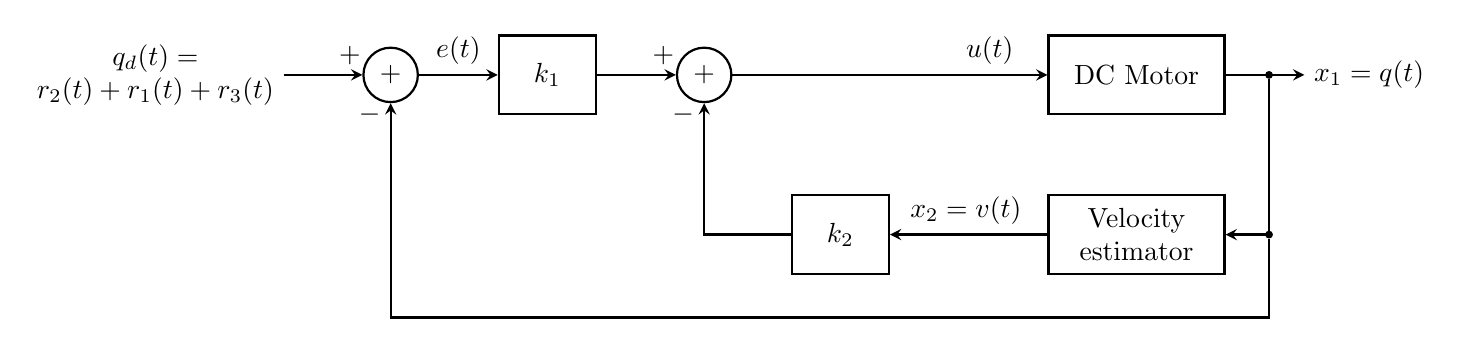
\begin{tikzpicture}[node distance = 10mm, auto]
	\node (Ref) [align=center] {$q_d(t)=$\\$r_2(t)+r_1(t)+r_3(t)$};
	\node (SummingPoint0) [draw,circle, thick, right = of Ref]  {+};
	\node(K1) [block, text width = 1cm, right= of SummingPoint0] {$k_1$};
	\node (SummingPoint1) [draw,circle, thick, right = of K1]  {+};
	\node(Plant) [block, text width = 2cm, right= 4cm of SummingPoint1] {DC Motor};
	\node (Out) [align=center, right = of Plant] {$x_1=q(t)$};
	\node(VelEst) [block, text width = 2cm, below= of Plant] {Velocity estimator};
	\node(K2) [block, text width = 1cm, left= 2cm of VelEst] {$k_2$};
	\node (PlantRight) [support, right = of Plant, right = 0.5cm, fill, circle,scale=0.3] {};
	\node (VelRight) [support, right = of VelEst, right = 0.5cm, fill, circle,scale=0.3] {};
	\node (VelRightDwn) [support, below = 1cm of VelRight] {};
	\draw [arrow] (Ref) -- (SummingPoint0) node[left=0.25cm, anchor=south east]{$+$};
	\draw [arrow] (SummingPoint0) -- node{$e(t)$} (K1);
	\draw [arrow] (K1) -- (SummingPoint1) node[left=0.25cm, anchor=south east]{$+$};
	\draw [arrow] (SummingPoint1) -- node[right=1.7cm, anchor=south east]{$u(t)$}(Plant);
	\draw [arrow] (Plant) -- (Out);
	\draw [arrow] (PlantRight) |- (VelEst);
	\draw [arrow] (VelEst) --  node[right=0.8cm, anchor=south east]{$x_2=v(t)$}(K2);
	\draw [arrow] (K2) -| (SummingPoint1) node[below=0.25cm, anchor=north east]{$-$};
	\draw [arrow] (VelRight) -- (VelRightDwn) -| (SummingPoint0) node[below=0.25cm, anchor=north east]{$-$};
\end{tikzpicture}
\caption{State feedback control}
\end{figure}




% ---- for the APP

\pagebreak
\begin{figure}
	\centering
	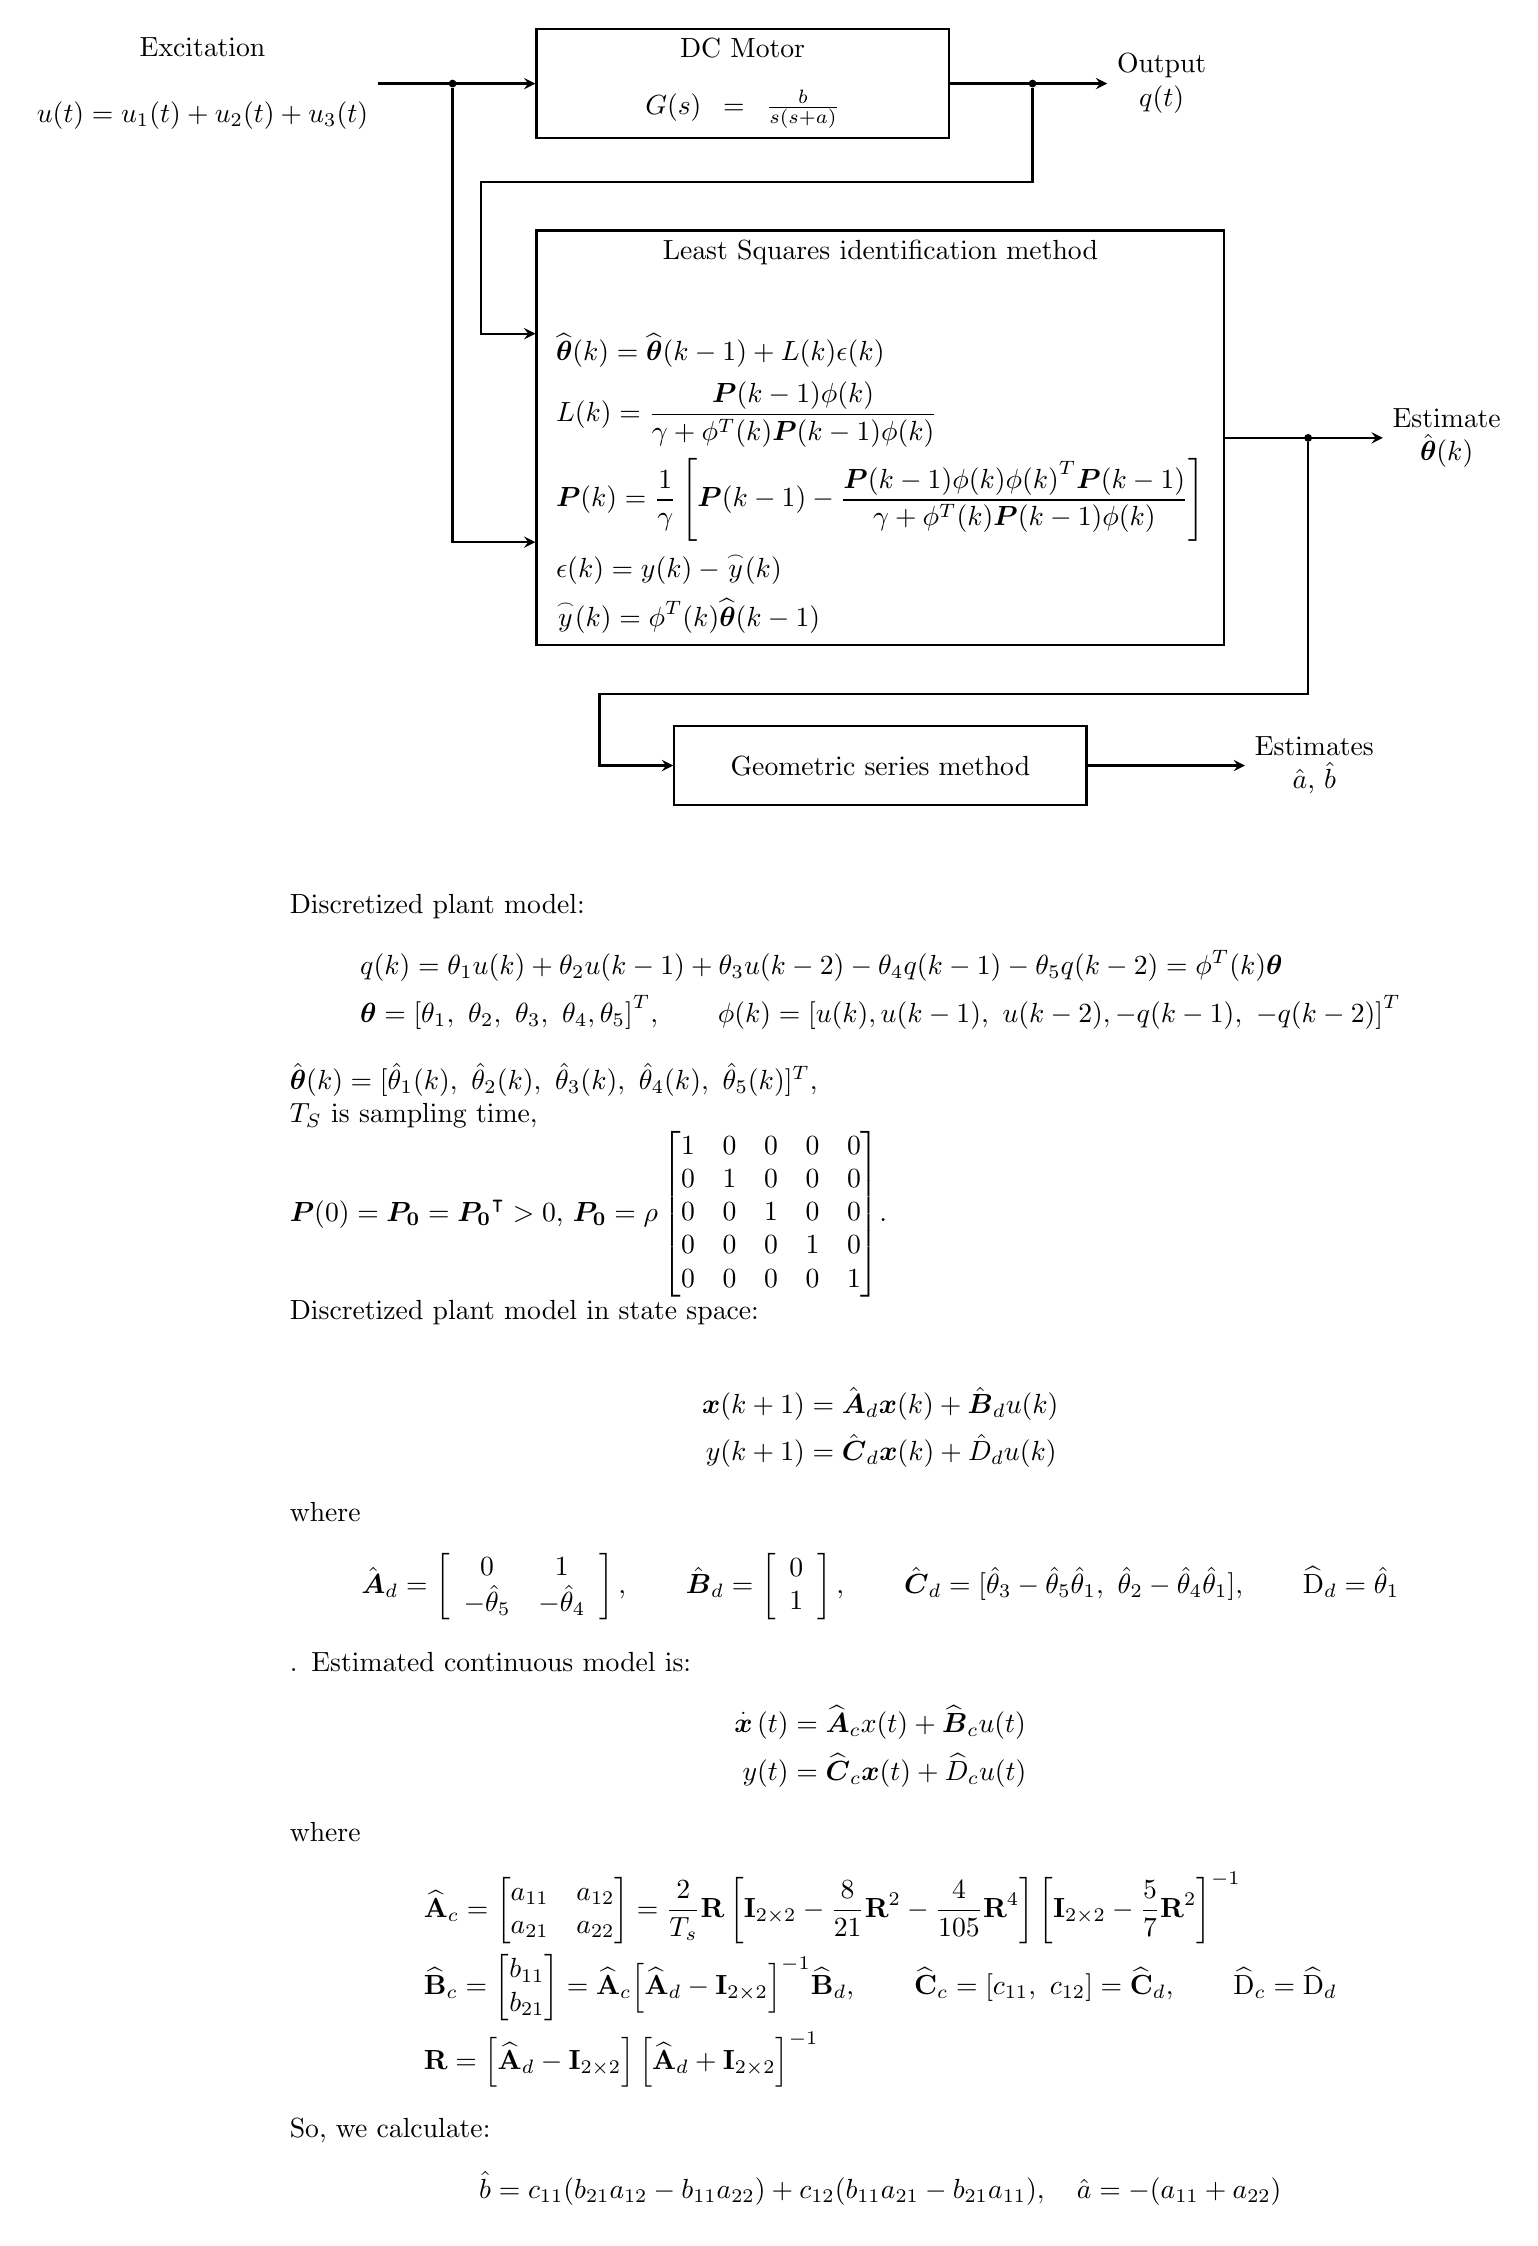
\begin{tikzpicture}[node distance = 10mm, auto]
		\node (Excitation) [align=center] {Excitation\\\\$u(t)=u_1(t)+u_2(t)+u_3(t)$};
		\node (Plant) [block, text width = 5cm, right = of Excitation, right = 2cm] {DC Motor \\[0.3cm] $G(s) = \frac{b}{s(s+a)}$};
		\node (PlantRight) [support, right = of Plant, right = 1cm, fill,circle,scale=0.3] {};
		\node (PlantLeft) [support, left = of Plant, left = 1cm, fill,circle,scale=0.3] {};
		\node (Identification) [block, text width = 8.5cm, below = 4.5 of Plant.west, anchor=west] {Least Squares identification method
			\\[0.1cm]
			\begin{align}
				& \widehat{\boldsymbol{\theta }}(k)=\widehat{\boldsymbol{\theta }}(k-1)+L(k)\epsilon (k) \nonumber\\
				& L(k)=\frac{\boldsymbol{P}(k-1)\phi (k)}{\gamma +{{\phi }^{T}}(k)\boldsymbol{P}(k-1)\phi (k)} \nonumber\\ 
				& \boldsymbol{P}(k)=\frac{1}{\gamma }\left[ \boldsymbol{P}(k-1)-\frac{\boldsymbol{P}(k-1)\phi (k)\phi {{(k)}^{T}}\boldsymbol{P}(k-1)}{\gamma +{{\phi }^{T}}(k)\boldsymbol{P}(k-1)\phi (k)} \right] \nonumber\\ 
				& \epsilon (k)=y(k)-\overset{\scriptscriptstyle\frown}{y}(k) \nonumber\\ 
				& \overset{\scriptscriptstyle\frown}{y}(k)={{\phi }^{T}}(k)\widehat{\boldsymbol{\theta }}(k-1)  \nonumber
			\end{align}
			
		};
		\node (IdentificationRight) [support, right = of Identification, right = 1cm, fill,circle,scale=0.3] {};
		\node (Geo) [block, text width = 5cm, below = 1 of Identification] {Geometric series method};
		\node (GeoOut) [right = of Geo, right = 2cm, align=center] {Estimates\\$\hat a$, $\hat b$};
		\node (Output) [right = of Plant, right = 2cm, align=center] {Output\\$q(t)$};
		\node (CapValues) [right = of Identification, right = 2cm, align=center] {Estimate\\$\hat{\boldsymbol{\theta}}(k)$};
		\path (Excitation.east) -- (Excitation.north east) coordinate[pos=0.5] (Reference1);
		\path (Identification.west) -- (Identification.north west) coordinate[pos=0.5] (Identification1);
		\path (Identification.west) -- (Identification.north west) coordinate[pos=-0.5] (Identification2);
		\path (Geo.west) -- (Geo.north west) coordinate[pos=0.0] (Geo1);
		\draw [arrow] (Excitation) -- (Plant);
		\draw [arrow] (Plant) -- (Output);
		\draw [arrow] (PlantRight) -- +(0, -1.25) -| +(-7,-1.25) |- (Identification1);
		\draw [arrow] (IdentificationRight) -- +(0, -3.25) -| +(-9,-3.25) |- (Geo1);
		\draw [arrow] (PlantLeft) |- (Identification2);
		\draw [arrow] (Identification) -- (CapValues);
		\draw [arrow] (Geo) -- (GeoOut);
		\node (Equation000) [text width = 15cm, below = 1cm of Geo, align = left] {
			Discretized plant model:
			\begin{align}
				& q(k)={{\theta }_{1}}u(k)+{{\theta }_{2}}u(k-1)+{{\theta }_{3}}u(k-2)-{{\theta }_{4}}q(k-1)-{{\theta }_{5}}q(k-2)={{\phi }^{T}}(k)\boldsymbol{\theta } \nonumber\\ 
				& \boldsymbol{\theta }={{[{{\theta }_{1}},\ {{\theta }_{2}},\ {{\theta }_{3}},\ {{\theta }_{4}},{{\theta }_{5}}]}^{T}},\qquad \phi (k)={{[u(k),u(k-1),\ u(k-2),-q(k-1),\ -q(k-2)]}^{T}} \nonumber
			\end{align}
			
			$\hat{\boldsymbol{ \theta}}(k)=[\hat{\theta}_{1}(k), \ \hat{\theta}_{2}(k), \ \hat{\theta}_{3}(k), \ \hat{\theta}_{4}(k), \ \hat{\theta}_{5}(k)]^{T}$,\\
			$T_S$ is sampling time, \\
			$\boldsymbol{P}(0) = \boldsymbol{P_0} = \boldsymbol{P_0}^\intercal>0$,
			$\boldsymbol{P_0} = \rho
			\begin{bmatrix}
				1 & 0 & 0 & 0 & 0 \\
				0 & 1 & 0 & 0 & 0 \\
				0 & 0 & 1 & 0 & 0 \\
				0 & 0 & 0 & 1 & 0 \\
				0 & 0 & 0 & 0 & 1 \\
			\end{bmatrix}$.\\
			Discretized plant model in state space:\\
			\begin{align}
				\boldsymbol{x}(k+1)&=\hat{\boldsymbol{A}}_{d}\boldsymbol{x}(k)+\hat{\boldsymbol{B}}_{d}u(k) \nonumber\\ 
				y(k+1)&=\hat{\boldsymbol{C}}_{d}\boldsymbol{x}(k) +\hat{{D}}_{d}u(k)\nonumber
			\end{align}\\
			where 
			\[\hat{\boldsymbol{A}}_{d}=\left[    
			\begin{array}{cc}
				0 & 1 \\
				-\hat{\theta}_{5} & -\hat{\theta}_{4}
			\end{array}
			\right], \qquad
			\hat{\boldsymbol{B}}_{d}=\left[    
			\begin{array}{c}
				0  \\
				1
			\end{array}
			\right], \qquad
			\hat{\boldsymbol{C}}_{d}=[{{\hat{\theta }}_{3}}-{{\hat{\theta }}_{5}}{{\hat{\theta }}_{1}},\ {{\hat{\theta }}_{2}}-{{\hat{\theta }}_{4}}{{\hat{\theta }}_{1}}],\qquad
			{{\widehat{\text{D}}}_{d}}={{\hat{\theta }}_{1}}\].
			Estimated continuous model is:
			\begin{align}
				\overset{.}{\mathop{\boldsymbol{x}}}\,(t)&={{\widehat{\boldsymbol{A}}}_{c}}x(t)+{{\widehat{\boldsymbol{B}}}_{c}}u(t) \nonumber \\ 
				y(t)&={{\widehat{\boldsymbol{C}}}_{c}}\boldsymbol{x}(t)+{{\widehat{{D}}}_{c}}u(t) \nonumber
			\end{align}
			where
			\begin{align}
				& {{\widehat{\mathbf{A}}}_{c}}=\left[ \begin{matrix}
					{{a}_{11}} & {{a}_{12}}  \\
					{{a}_{21}} & {{a}_{22}}  \\
				\end{matrix} \right]=\frac{2}{{{T}_{s}}}\mathbf{R}\left[ {{\mathbf{I}}_{2\times 2}}-\frac{8}{21}{{\mathbf{R}}^{2}}-\frac{4}{105}{{\mathbf{R}}^{4}} \right]{{\left[ {{\mathbf{I}}_{2\times 2}}-\frac{5}{7}{{\mathbf{R}}^{2}} \right]}^{-1}} \nonumber\\ 
				& {{\widehat{\mathbf{B}}}_{c}}=\left[ \begin{matrix}
					{{b}_{11}}  \\
					{{b}_{21}}  \\
				\end{matrix} \right]={{\widehat{\mathbf{A}}}_{c}}{{\left[ {{\widehat{\mathbf{A}}}_{d}}-{{\mathbf{I}}_{2\times 2}} \right]}^{-1}}{{\widehat{\mathbf{B}}}_{d}},\qquad {{\widehat{\mathbf{C}}}_{c}}=[{{c}_{11}},\ {{c}_{12}}]={{\widehat{\mathbf{C}}}_{d}},\qquad {{\widehat{\text{D}}}_{c}}={{\widehat{\text{D}}}_{d}} \nonumber\\ 
				& \mathbf{R}=\left[ {{\widehat{\mathbf{A}}}_{d}}-{{\mathbf{I}}_{2\times 2}} \right]{{\left[ {{\widehat{\mathbf{A}}}_{d}}+{{\mathbf{I}}_{2\times 2}} \right]}^{-1}} \nonumber
			\end{align}
			So, we calculate:
			\begin{align}
				& {{{\hat{b }}}}={{c}_{11}}({{b}_{21}}{{a}_{12}}-{{b}_{11}}{{a}_{22}})+{{c}_{12}}({{b}_{11}}{{a}_{21}}-{{b}_{21}}{{a}_{11}}),\quad {{{\hat{a }}}}=-({{a}_{11}}+{{a}_{22}}) \nonumber 
			\end{align}
			
		};
	\end{tikzpicture}
	\caption{Identification of the DC motor parameters}
\end{figure}

\begin{figure}
	\centering
	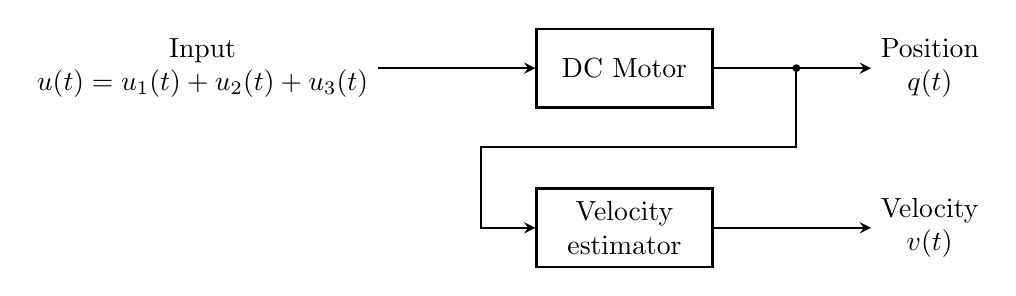
\begin{tikzpicture}[node distance = 10mm, auto]
		\node (Input) [align=center] {Input\\$u(t)=u_1(t)+u_2(t)+u_3(t)$};
		\node (Plant) [block, text width = 2cm, right = 2cm of Input] {DC Motor};
		\node (Output) [right = of Plant, right = 2cm, align=center] {Position\\$q(t)$};
		\node (VelEst) [block, text width = 2cm, below = 1 of Plant] {Velocity\\estimator};
		\node (VelOut) [right = of VelEst, right = 2cm, align=center] {Velocity\\$v(t)$};
		\node (PlantRight) [support, right = of Plant, right = 1cm, fill,circle,scale=0.3] {};
		\path (VelEst.west) -- (VelEst.north west) coordinate[pos=0.0] (VelEst1);
		\draw [arrow] (Input) -- (Plant);
		\draw [arrow] (Plant) -- (Output);
		\draw [arrow] (VelEst) -- (VelOut);
		\draw [arrow] (PlantRight) -- +(0, -1) -| +(-4,-1) |- (VelEst1);
	\end{tikzpicture}
	\caption{Open loop system}
\end{figure}






\begin{figure}
	\centering
	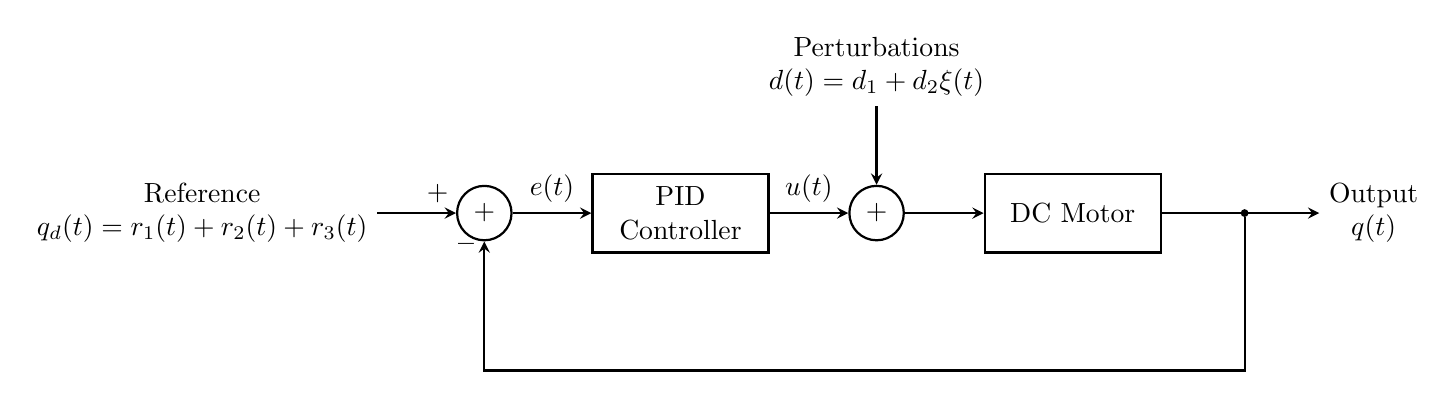
\begin{tikzpicture}[node distance = 10mm, auto]
		\node (Reference) [align=center] {Reference\\$q_d(t)=r_1(t)+r_2(t)+r_3(t)$};
		\node (SummingPoint) [draw,circle, thick, right = of Reference]  {+};
		\node (Control) [block, text width = 2cm, right = of SummingPoint] {PID Controller};
		\node (SummingPoint1) [draw,circle, thick, right = of Control]  {+};
		\node (Plant) [block, text width = 2cm, right = of SummingPoint1] {DC Motor};
		\node (PlantRight) [support, right = of Plant, right = 1cm, fill, circle,scale=0.3] {};
		\node (Output) [right = of Plant, right = 2cm, align=center] {Output\\$q(t)$};
		\node (Perturbations) [align=center, above = of SummingPoint1] {Perturbations\\$d(t)=d_1+d_2\xi(t)$};
		\draw [arrow] (Reference) -- node[anchor=south west]{+}(SummingPoint);
		\draw [arrow] (SummingPoint) -- node[anchor=south]{$e(t)$}(Control);
		\draw [arrow] (Control) -- node[anchor=south]{$u(t)$}(SummingPoint1);
		\draw [arrow] (SummingPoint1) -- (Plant);
		\draw [arrow] (Plant) -- (Output);
		\draw [arrow] (PlantRight) -- +(0, -2) -| (SummingPoint) node[below = 2mm, anchor=north east]{\bf\textendash};
		\draw [arrow] (Perturbations) -- (SummingPoint1);
	\end{tikzpicture}
	\caption{Closed loop system with a PID Controller}
\end{figure}


\begin{figure}
	\centering
	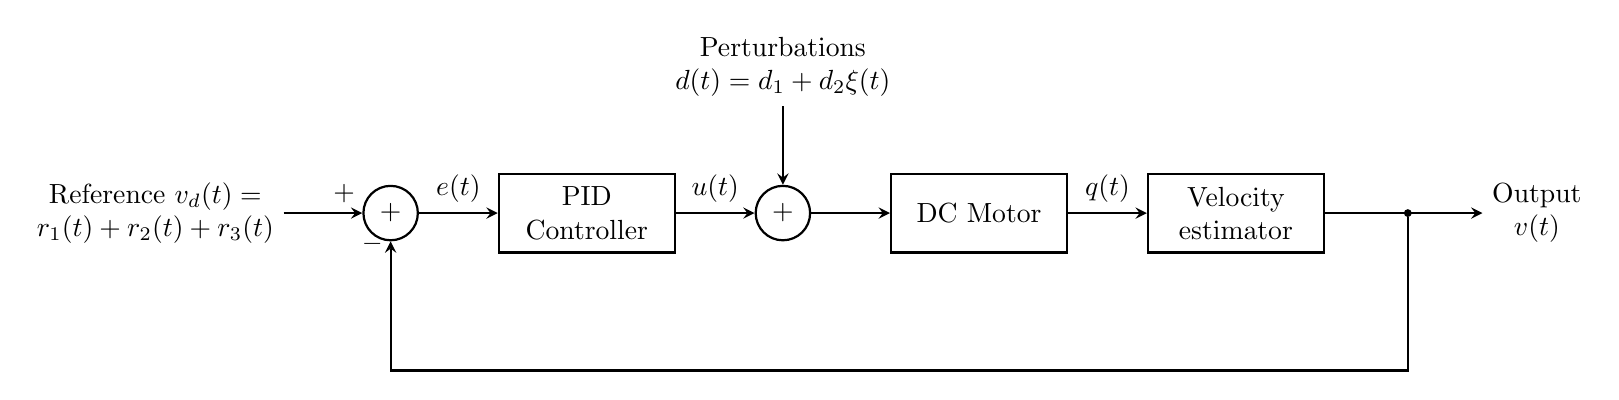
\begin{tikzpicture}[node distance = 10mm, auto]
		\node (Reference) [align=center] {Reference $v_d(t)=$\\$r_1(t)+r_2(t)+r_3(t)$};
		\node (SummingPoint) [draw,circle, thick, right = of Reference]  {+};
		\node (Control) [block, text width = 2cm, right = of SummingPoint] {PID Controller};
		\node (SummingPoint1) [draw,circle, thick, right = of Control]  {+};
		\node (Plant) [block, text width = 2cm, right = of SummingPoint1] {DC Motor};
		\node (VelEst) [block, text width = 2cm, right = of Plant] {Velocity\\estimator};
		\node (VelRight) [support, right = of VelEst, right = 1cm, fill, circle,scale=0.3] {};
		\node (Output) [right = of VelEst, right = 2cm, align=center] {Output\\$v(t)$};
		\node (Perturbations) [align=center, above = of SummingPoint1] {Perturbations\\$d(t)=d_1+d_2\xi(t)$};
		\draw [arrow] (Reference) -- node[anchor=south west]{+}(SummingPoint);
		\draw [arrow] (SummingPoint) -- node[anchor=south]{$e(t)$}(Control);
		\draw [arrow] (Control) -- node[anchor=south]{$u(t)$}(SummingPoint1);
		\draw [arrow] (SummingPoint1) -- (Plant);
		\draw [arrow] (Plant) -- node[anchor=south]{$q(t)$}(VelEst);
		\draw [arrow] (VelEst) -- (Output);
		\draw [arrow] (VelRight) -- +(0, -2) -| (SummingPoint) node[below = 2mm, anchor=north east]{\bf\textendash};
		\draw [arrow] (Perturbations) -- (SummingPoint1);
	\end{tikzpicture}
	\caption{Closed loop system with a PID Controller}
\end{figure}



\begin{figure}
	\centering
	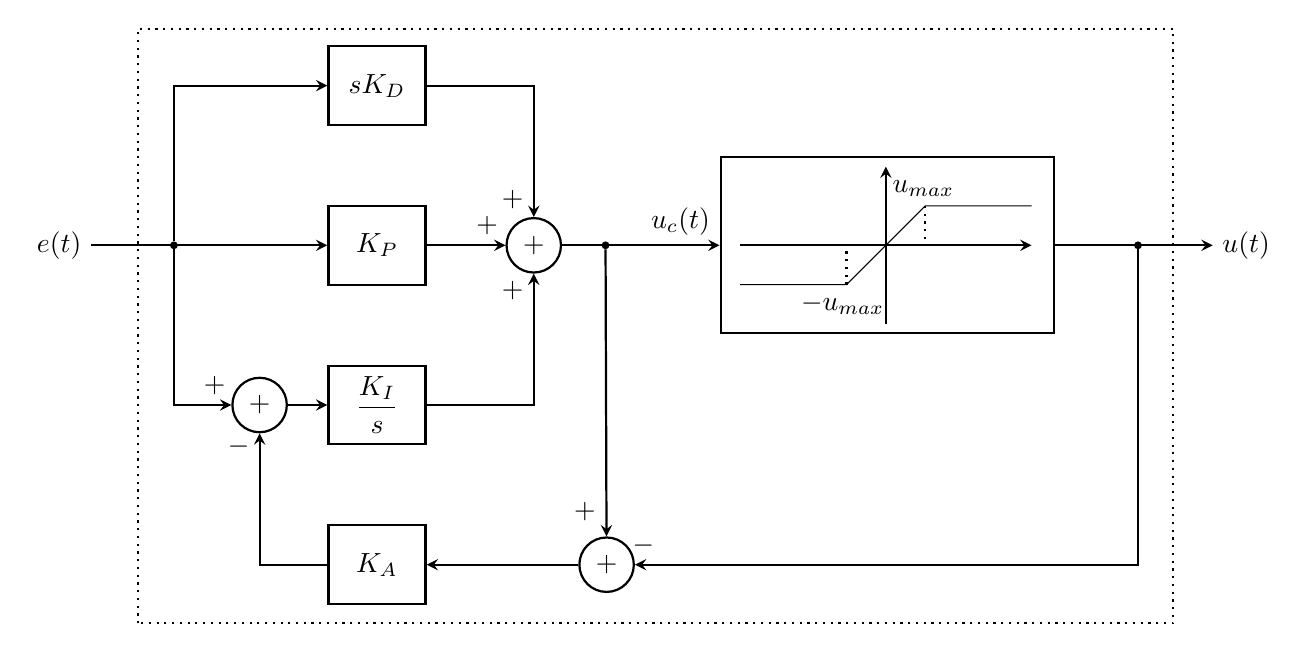
\begin{tikzpicture}[node distance = 10mm, auto]
		\node (Error) [align=center] {$e(t)$};
		\node (KP) [block, text width = 1cm, right = 3cm of Error] {$K_P$};
		\node (KD) [block, text width = 1cm, above = of KP] {$sK_D$};
		\node (KI) [block, text width = 1cm, below = of KP] {$\dfrac{K_I}{s}$};
		\node (KA) [block, text width = 1cm, below = of KI] {$K_A$};
		\node (SummingPoint0) [draw,circle, thick, right = of KP]  {+};
		\node (SummingPoint1) [draw,circle, thick, left = 0.5cm of KI]  {+};
		\node (SummingPoint2) [draw,circle, thick, right = 1.925cm of KA]  {+};
		\node (Sat) [block, text width = 4cm, text height = 2cm, right = 2cm of SummingPoint0] {};
		\node (Out) [align=center, right = 2cm of Sat] {$u(t)$};
		\node (ErrorRight) [support, right = of Error, right = 1cm, fill, circle,scale=0.3] {};
		\node (SummingPoint0Right) [support, right = of SummingPoint0, right = 0.5cm, fill, circle,scale=0.3] {};
		\node (SatRight) [support, right = of Sat, right = 1cm, fill, circle,scale=0.3] {};
		\draw [arrow] (Error) -- (KP);
		\draw [arrow] (ErrorRight) |- (KD);
		\draw [arrow] (ErrorRight) |- node[right = 0.25cm, anchor=south west]{$+$}(SummingPoint1);
		\draw [arrow] (SummingPoint1) -- (KI);
		\draw [arrow] (KA) -| node[above = 1.75cm, anchor=north east]{$-$}(SummingPoint1);
		\draw [arrow] (KP) -- node[anchor=south west]{$+$}(SummingPoint0);
		\draw [arrow] (KD) -| node[below=1.2cm, anchor=north east]{$+$}(SummingPoint0);
		\draw [arrow] (KI) -| node[above=1.2cm, anchor=south east]{$+$}(SummingPoint0);
		\draw [arrow] (SummingPoint0) -- node[anchor=south west]{$u_c(t)$}(Sat);
		\draw [arrow] (SummingPoint0Right) -- node[below=1.75cm, anchor=south east]{$+$}(SummingPoint2);
		\draw [arrow] (SummingPoint2) -- (KA);
		\draw [arrow] (Sat) -- (Out);
		\draw [arrow] (SatRight) |- (SummingPoint2)  node[ right =0.2cm, anchor=south west]{$-$};
		\draw [arrow] (8.65,0)  -- (12.35,0);
		\draw [arrow] (10.5,-1)  -- (10.5,1);
		\draw (8.65,-0.5) node [right=1.3cm, anchor= north] {$-u_{max}$}  -- (10.0,-0.5) -- (11,0.5) -- node [left=0.7cm, anchor= south] {$u_{max}$} (12.35,0.5);
		\draw [dotted, thick] (10.0,-0.5) -- (10.0,0);
		\draw [dotted, thick] (11.0,0.5) -- (11.0,0);
		\draw [dotted, thick] (1,-4.8) -- (1,2.75) -- (14.15,2.75) -- (14.15,-4.8) -- (1, -4.8);
	\end{tikzpicture}
	\caption{PID Controller with anti-windup}
\end{figure}


\begin{figure}
	\centering
	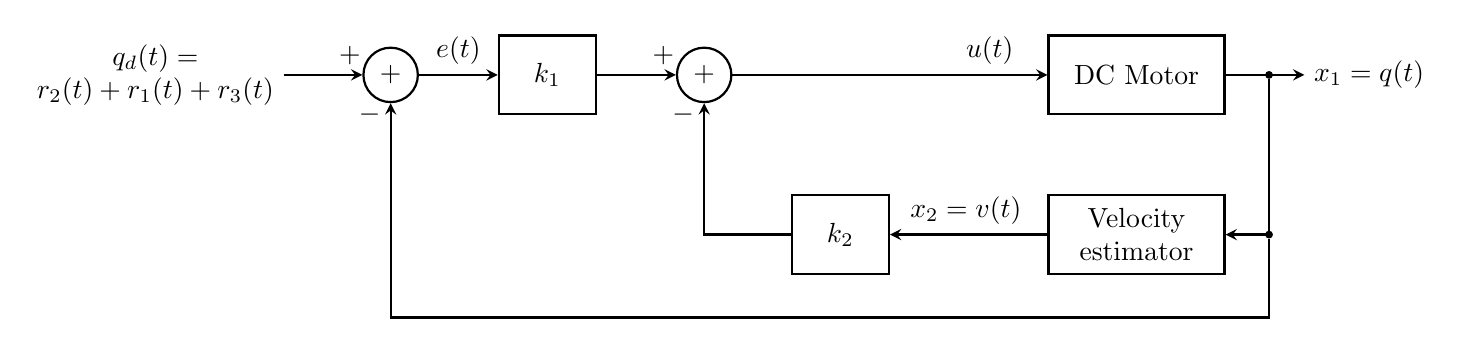
\begin{tikzpicture}[node distance = 10mm, auto]
		\node (Ref) [align=center] {$q_d(t)=$\\$r_2(t)+r_1(t)+r_3(t)$};
		\node (SummingPoint0) [draw,circle, thick, right = of Ref]  {+};
		\node(K1) [block, text width = 1cm, right= of SummingPoint0] {$k_1$};
		\node (SummingPoint1) [draw,circle, thick, right = of K1]  {+};
		\node(Plant) [block, text width = 2cm, right= 4cm of SummingPoint1] {DC Motor};
		\node (Out) [align=center, right = of Plant] {$x_1=q(t)$};
		\node(VelEst) [block, text width = 2cm, below= of Plant] {Velocity estimator};
		\node(K2) [block, text width = 1cm, left= 2cm of VelEst] {$k_2$};
		\node (PlantRight) [support, right = of Plant, right = 0.5cm, fill, circle,scale=0.3] {};
		\node (VelRight) [support, right = of VelEst, right = 0.5cm, fill, circle,scale=0.3] {};
		\node (VelRightDwn) [support, below = 1cm of VelRight] {};
		\draw [arrow] (Ref) -- (SummingPoint0) node[left=0.25cm, anchor=south east]{$+$};
		\draw [arrow] (SummingPoint0) -- node{$e(t)$} (K1);
		\draw [arrow] (K1) -- (SummingPoint1) node[left=0.25cm, anchor=south east]{$+$};
		\draw [arrow] (SummingPoint1) -- node[right=1.7cm, anchor=south east]{$u(t)$}(Plant);
		\draw [arrow] (Plant) -- (Out);
		\draw [arrow] (PlantRight) |- (VelEst);
		\draw [arrow] (VelEst) --  node[right=0.8cm, anchor=south east]{$x_2=v(t)$}(K2);
		\draw [arrow] (K2) -| (SummingPoint1) node[below=0.25cm, anchor=north east]{$-$};
		\draw [arrow] (VelRight) -- (VelRightDwn) -| (SummingPoint0) node[below=0.25cm, anchor=north east]{$-$};
	\end{tikzpicture}
	\caption{State feedback control}
\end{figure}





\end{document}